\section{Model and data description}
Our main goal is to predict whether companies would collapse next year using both ranking information and a network similarity product. Jing Fang et al \cite{fan2018combined} introduced this network and the task, and we follow them by integrating their task into a GCN formalism for each year, and testing whether combing GCNs from multiple years under one combined LSTM outperforms a GCN for each time point (TP).

The advantage of such a formalism is the possibility of using information from previous years to improve the accuracy of the prediction this year. Another advantage is the production of a single GCN for all years leading to a simpler interpretation of the results. We show here that the proposed approach does improve the average accuracy. 

Formally our model is as follows, Given a set of TP: $TP=1 \to k$ and for each time point we are given an undirected graph represented by an adjacency matrix $A^k$, a label for each node $i$ in the graph $z_{k}(i)$ and possibly some external input on each node $\vec{x}_{k}(i)$. We use a GCN $H^k$ to classify the labels using either only the graph topology or a combination of the graph topology and the external input. We then tested multiple methods to represent the graph topology and computed the resulting accuracy. We then test whether using the GCN output as the input to a LSTM and learning the labels using the LSTM produces a higher accuracy. We tested 4 configurations:
\begin{itemize}
\item   Pure GCN model on each year – yielding $n$ models - one for each snapshot (year) to predict the outcome in the following snapshot (i.e. prediction from the interactions in year $k$ the collapse of the company in year $k+1$).
\item   Pure GCN model trained on all years simultaneously – yielding a single model, compatible for all snapshots (i.e. shared weights between the GCN of all years). This model was trained in each TP. Thus at each TP, we recompute the model over all previous TP.
\item   Two phases models, where we first train the single model learned (as above), and then we use it’s one before the last layer as the input to an RNN.
\item   A combined model where the combined GCN and RNN are trained simultaneously.
\end{itemize}

\subsection {Different static model for each year}
We extended the GCN model developed by Thomas Kipf et al. \cite{kipf2016semi}. Each GCN layer is defined as: $$X_{n+1}=\sigma(A*X_{n}*W_n)$$ where $A$ is the adjacency matrix, $X$ is the input from the previous layer, and $W$ are the weights of the current layer. The activation function for intermediate layers was the ReLu function, and the last layer was linear. Dropout rates of 40\% and $L2$ regularization with a weight of 0.001 were used. The models were trained for 200 epochs with a Negative-Log-Likelihood loss on a weighted distribution of classes (to correct the imbalanced distribution of labels) and an Adam optimizer. The GCN had three internal layers of sizes 100 and 35 and 20 in all models studied. The main difference between the current model and existing GCN is the usage of a topology or neighbors' tags as input to the nodes. In the absence of any external information on the nodes, we propose to use one of the two possible inputs: A) Characterize each node by a vector of topological attributes, and use this vector as an input, B) Compute the number of neighbors and second neighbors that have a given tag and use this number as the input layer of the GCN. This creates a vector of twice the number of possible tags for each node. When external information is available we introduce the external information and topological

%The extension comes through the incorporation of an asymmetric adjacency matrix. In this model we do not lose the direction of the graph, which contains topological information. We incorporate the direction by taking the adjacency matrix (asymmetric in directed graph) and concatenate its transpose to it – creating a$ 2n x n$ adjacency matrix. The dimension of the output of each layer is: $[(2NxN)*(Nxi_n )*(i_n xo_n )]=2Nxo_n$., which in turn is passed to the next layer following a rearrangement of the output by splitting and concatenating it to change dimensions from  - $2NxO_n$  to $ Nx2O_n$. 

%At first, we wanted to asses our data on the base model (MultiLayerGCN and CombinedGCN). In this stage, we performed complete learning of the base model on each of the snapshots, independently of each other. Both these base models support directed graphs and undirected graphs using a symmetric or an asymmetric version correspondingly.

\subsection{Combined static model for all the years}
We used the two basic models above (with and without external information) and trained each of them on all snapshots simultaneously. Unlike the previous stage, the process yields unified models that are learned and tested over all the snapshots together. So, the only difference between this approach and the previous is weight sharing between the $TP$. The models were again trained for 200 epochs with a Negative-Log-Likelihood loss on a weighted distribution of classes and an Adam optimizer. In both approaches (shared and distinct weights), the only parameter that was varied was the $L2$ regularization and values between $1.e-4$ and $1.e-1$ were tested in $log10$ jumps of 1 log. All results are presented as the average of 3 runs, and the resulting standard error.

\subsection{ Two-phase model – with separate GCN and RNN}
In this model, the GCN was combined with an RNN that handles the network dynamics. First, we trained the unified model for all the years as above. This unified model still represents a static approach for the classification. We then trained the RNN. The input for the RNN layer was the one before the last layer of the static model. To do so, we forward propagated each TP through the static part of the model, so that the input of the second phase is of dimensions $[N_{seq}xN_{nodes}*O_{l-1}]$ where $N_{seq}=17$ – the sequence length (number of snapshots), $N_{nodes}$– the number of nodes in the complete unified graph, and $O_{l-1}=20$, the chosen size of the layer before the last in the static part. This model was trained as described above, and the RNN was trained using a cross-entropy loss with quadratic loss function and an LBFGS optimizer.

\subsection{Fully combined model}
If in the previous model, we trained two distinct models (a static GCN and an RNN) one after the other while passing the output from the GCN model as an input to train the other model. Here, we built a single model to handle both through a combined backpropagation. Each snapshot is propagated through the GCN with a slight difference that the last layer is not the number of classes, but the size of the layer before the last (as described in the model above). The RNN internal state was initialized with zeros for each node, and the RNN output a vector of the size of classes for each node in each snapshot, which was compared to a log-softmax function. We used the Negative-Log-Likelihood loss function, and like the model above, we also used the LBFGS optimizer.

\subsection{Networks studied}
% For ease of use, all graphs in time must contain the same nodes (different edges), so we need to “pad” each graph with the missing nodes. At first, we checked how many nodes are changing along with the various graphs – added and removed nodes.
% We collect all the nodes of all the graphs of the different snapshots (identified by their IDs), and for each graph, we add the missing nodes from the collected group (without any labeling).
% The split of the nodes occurs once at the beginning on the entire set of nodes, and for each graph, the train-Val-test are taken from this split. The train set is an intersection of the train part of the split and the labeled nodes.
We used the company similarity networks introduced by JingFang et al \cite{fan2018combined}. These networks represent product similarity between companies between 1996 and 2012. Shortly, for each pair of companies, the overlap in their product description was computed (using a Jaccard-Index over product categories), leading to a similarity network between companies. Following the same analysis, for each company, external measures from its balance sheets were also used, including the total balance, rating, etc). We predict here using the network and external features whether the company would bankrupt the following year. The average area under the curve (AUC) obtained by Jing-Fang et al over all years was 0.62.
\\For ease of use, all graphs were zero-padded to contain the same number of nodes The split of nodes into training and test sets was performed once at the beginning on the entire set of nodes and was the same for each TP. The training set is an intersection of the train part of the split and the labeled nodes (since some nodes are not labeled in some TP). We here used a constant train fraction of 60\% and 20\% internal validation, following again the work of Jing Fang et al.
\\To further test the GCN-LSTM and the introduction of topology, we studied a network with no external input on the nodes. This dataset captures the activity of users of a medium-sized social news aggregation website similar to reddit.com or Y Combinator’s hacker news. These users collect and post news from around the web, rank and discuss these posts creating threads of comments, up-vote and down-vote comments of other users. The web site encourages users to maintain two kinds of social networks: they can express their attitude towards any other user (i.e. users can indicate whether they like, neutral or dislike any registered user thus revealing their attitude and implicitly affecting the reputation of the target user) and they can create directed friendship links. Both social networks are quite dynamic and change in response to activities such as publication or support of certain posts expressed opinions or even the establishment of friendship relationship with other peers. The web site operator shared anonymous data about user activity – the posts, up and down-votes of the posts and comments as well as several snapshots of relationship and friendship statuses that allowed us to reconstruct the social network. From the full set of users, we built a directed graph where the nodes are the users, and the directed edges are the following status. (directed friendships), producing 11 directed graphs. On each graph, we checked for each user whether the number of posted stories was higher than 3, and this was the activity measure we wanted to predict.

\begin{figure}[h!]
    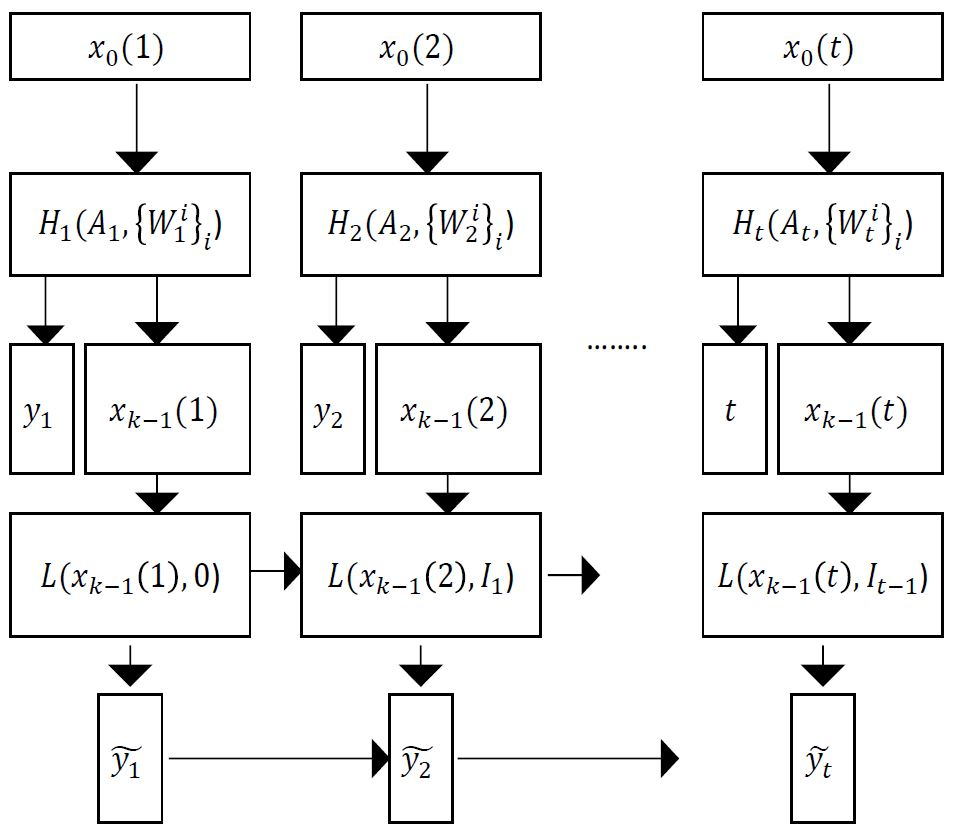
\includegraphics[width=\textwidth]{model}
    \centering
    \caption{\textit{Model description. The observations are input for all the nodes in the network for every TP $x_{0}(t)$ and a class for each node in each TP $z_{t}$. $x_{0}(t)$ is the input to a GCN $H_{t}$ that is based on the network in the TP $A_{t}$. We extract from the GCN the output values $y_{t}$ and the one before last layer $x_{k-1}(t)$. This layer is fed to an LSTM L which passed internal states and output to the following TP and produced a classification for each node in each time point $\tilde{y}_{t}$. In the first model, only the GCN was used and $y_{t}$ was compared to $z_{t}$. In the second model, the same analysis was performed, but the weights were shared among the $H_{t}$. In the following models, weights were still shared, but the comparison was between $\tilde{y}_{t}$ and $z_{t}$, The only difference between the third and fourth models is in the training. In the third model $H$ and $L$ were trained separately, and in the forth they were trained simultaneously.}}
    \label{fig:model}
\end{figure}